\subsection{Das ,,fertige`` Produkt}\label{ku_produkt}
\begin{figure}[h!t]
	
\includegraphics[width=1\textwidth]{img/placeholder.png}
	\caption[Smart Home Zentrale]{Smart Home Zentrale}
	\label{fig:smart-home-zentrale}
\end{figure}
\noindent Dies ist das Ergebnis der Technikerarbeit von Felix Kuschel und Manuel Starz. 
Eine Smart Home Zentrale auf Basis von Homeassistant mit einer ZigBee-Antenne, einem 10.1'' großen Touchbildschirm und der Möglichkeit, per LAN und WLAN mit dem Heimnetz in Verbindung zu treten.\par
\noindent Das Gehäuse ist für die Wand-Montage konzipiert, die Nutzung eines Gehäuse um die Smart Home Zentrale auf einer Kommode oder in einem Regal zu platzieren (mit einem leichten Winkel) ist ebenfalls möglich. (vgl. \ref{fig:case-with-feet})
\begin{figure}[h!tb]
	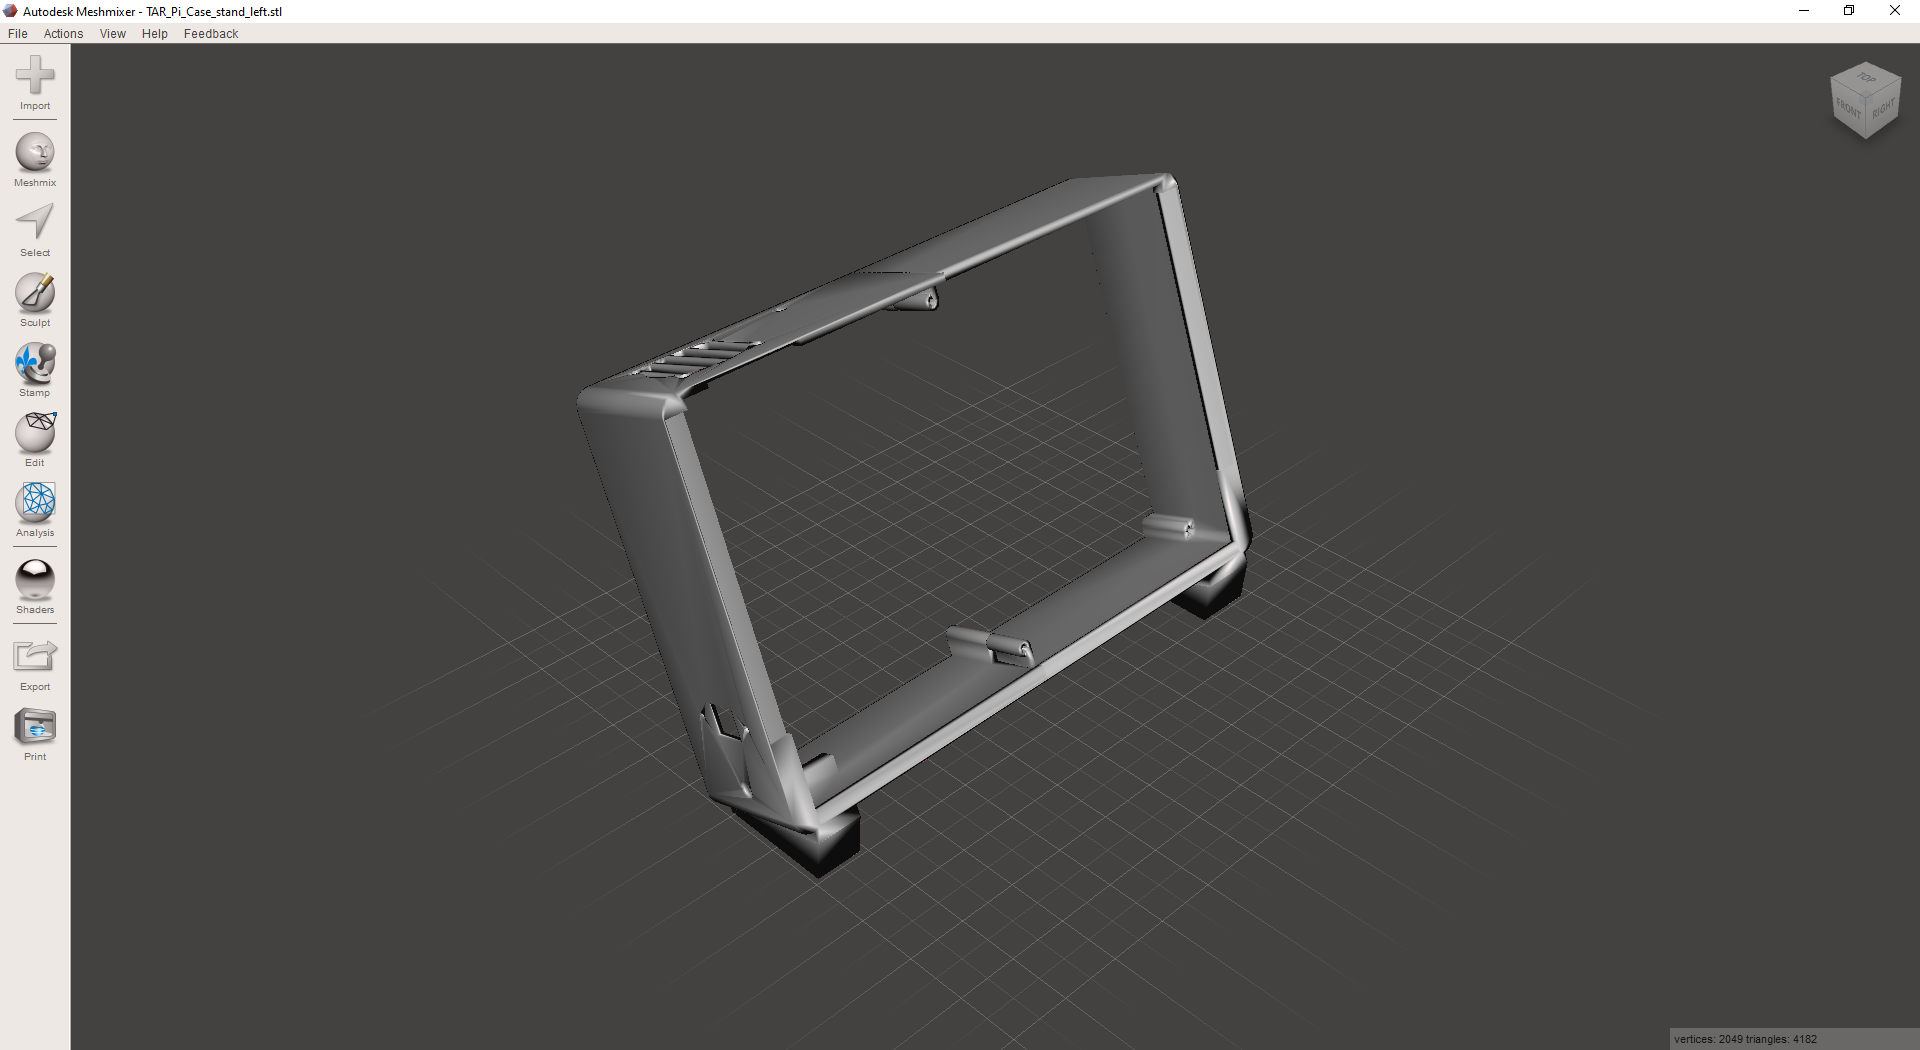
\includegraphics[width=1\textwidth]{img/stand_case.png}
	\caption[Gehäuse mit Füßen (Render in Meshmixer)]{Gehäuse mit Füßen (Render in Meshmixer)}
	\label{fig:case-with-feet}
\end{figure}